\documentclass{article}
\usepackage{cmap}
\usepackage[T2A]{fontenc}
\usepackage[utf8]{inputenc}
\usepackage[english,russian]{babel}
\usepackage{setspace}
\usepackage{geometry}
\usepackage{graphicx}
\usepackage{amsfonts}
\graphicspath{{graphicslab4/}}
\DeclareGraphicsExtensions{.pdf, .png, .jpg, .fig}
\geometry{top=2cm}
\geometry{bottom=2cm}
\geometry{left=2cm} % отступ справа
\geometry{right=2cm} % отступ слева

\begin{document}
	\begin{center}
		\hfill \break
		\begin{center}
			\huge{Санкт-Петербургский политехнический университет\\
				Высшая школа прикладной математики\\
				и вычислительной физики, ФизМех}
		\end{center}
		\hfill \break
		\hfill \break
		\hfill \break
		\hfill \break
		\hfill \break
		\huge{Направление подготовки\\
			«Прикладная математика и информатика»}\\
		\hfill \break
		\hfill \break
		\hfill \break
		\hfill \break
		\hfill \break
		\hfill \break
		\fontsize{14pt}{14pt}\selectfont
		Отчет по лабораторной работе №4\\
		«Решение алгебраической проблемы собственных значений итерационными методами»\\
		\hfill \break
		\hfill \break
		\hfill \break
		\hfill \break
		\hfill \break
	\end{center}
	\hfill \break
	\hfill \break
	\fontsize{12pt}{12pt}\selectfont
	\begin{tabular}{cccc}
		\hspace{1cm}Выполнил студент гр. 5030102/00003 & {\hspace{3cm}} & & Петрошенко А.В. \\\\
		\hspace{-3cm}Преподаватель: &{\hspace{1cm}}& & {\hspace{1cm}} Курц В.В. \\\\
	\end{tabular}\\
	\hfill \break
	\hfill \break
	\hfill \break
	\hfill \break
	\hfill \break
	\hfill \break
	\begin{center} Санкт-Петербург\\ 
		2021\\
	\end{center}
	\thispagestyle{empty}
	\newpage
	\begin{center} \textbf{Формулировка задачи и ее формализация}\end{center}
	Собственные числа и собственные вектора(далее СЧ и СВ) - основные характеристики матрицы, поэтому их нахождение является важной задачей вычислительной математики. Методы нахождения можно разделить на те, которые решают полную задачу, то есть находят все СЧ и СВ, и на те, коорые решают эту задачу частично, то есть находят, например, только максимальное СЧ.\\ В данной работе будет реализован метод, который ищет максимальное СЧ и соответствующий ему СВ.\\
	\\
	\underline{Постановка задачи:}\\
	Дана матрица $A \in \mathbb{R} ^{n \times n}$, требуется найти такой $\lambda_{max}$ и такой $x$, что $A\lambda_{max} = \lambda_{max}x$, где $\lambda_{max}$ - не равен 0 и $x$ - не нулевой вектор.\\
	Матрица размерности $n \times n$ имеет $n$ СЧ и СВ.\\
	В данной работе будет реализован степенной метод с нормировкой и со сдвигами для улучшения его сходимости.
	\begin{center} \textbf{Алгоритм метода и условия его применимости}\end{center}
	Величина $|\frac{\lambda_2}{\lambda_1}|$ определяет скорость сходимости: чем она меньше, тем быстрее сходится. Поэтому для уменьшения данной величины сдвинем все собственные числа на $\mu = \frac{\lambda_2 + \lambda_n}{2}$ - это оптимальный сдвиг\\
	Далее реализуем сам степенной метод с нормировкой для данного сдвига, то есть для матрицы $B = A - \mu E$\\
	\underline{Алгоритм метода:}\\
	\begin{enumerate}
		\item Берем произвольный вектор $y_0 \in \mathbb{R}^n$ и нормируем его:\\
		$\overline{y}_0 = \frac{y_0}{\mu_0}$, $\mu_0 = y^0_s$, $y^0_s = ||y_0||_{\infty}$
		\item Реализуем итерационную последовательность:\\
		$y_k = A\overline{y}_{k-1}$, $\overline{y}_k = \frac{y_k}{\mu_k}$, $\mu_k = y^k_s$, $y^k_s = ||y_k||_{\infty}$
	\end{enumerate}
	Для окончания итерационного процесса будем использовать апостериорную оценку:
	$$\frac{||A\overline{y}_k - \mu_k \overline{y}_k||_2}{||\overline{y}_k||_2} \geq \epsilon$$
	Получаем, что $\mu_k \rightarrow \lambda_1$, $\overline{y}_k \rightarrow \alpha w_1$\\
	Мы получили СЧ и СВ матрицы $B$, СЧ матрицы $A$ будет равен найденному СЧ плюс выбранный нами сдвиг, а собственные вектора матриц $A$ и $B$ равны.
	\underline{Условия применимости метода:}\\
	$A$ - вещественная положительно определенная матрица, у которой 2 максимальных по модулю собственных числа различны.
	\begin{center} \textbf{Предварительный анализ задачи}\end{center}
	АПСЗ наиболее устойчива в случае, когда $A = A^T$. Таким образом, нам нужно задать положительно определенную симметричную матрицу: $A = QDQ^T$, где $Q$ - ортогональная матрица, а $D$ - диагональная. Теперь также удобно задавать отделимость собсвенных чисел.
	\begin{center} \textbf{Тестовый пример для задач малой размерности}\end{center}
	Возьмем ортогональную матрицу: $Q = \left(
	\begin{array}{ccc}
		-0.9812  &  0.1729  &  0.0854\\
		-0.1762  & -0.6237  & -0.7615\\
		-0.0784  & -0.7623  &  0.6425
	\end{array}
	\right)$, $D = \left(
	\begin{array}{ccc}
		1  &  0  &  0\\
		0  &  2  &  0\\
		0  &  0  &  3
	\end{array}
	\right)$\\
	\\
	Тогда $A = \left(
	\begin{array}{ccc}
		1.0444  & -0.2379  & -0.0221\\
		-0.2379  &  2.5487  & -0.5031\\
		-0.0221  & -0.5031  &  2.4068
	\end{array}
	\right)$\\
	Матрица $B = A - \mu E = \left(
	\begin{array}{ccc}
		-0.4556  & -0.2379  & -0.0221\\
		-0.2379  &  1.0487  & -0.5031\\
		-0.0221  & -0.5031  &  0.9068
	\end{array}
	\right)$
	Возьмем $y_00 = \left(
	\begin{array}{c}
		1\\
		1\\
		1
	\end{array}
	\right)$ и найдем решение с точностью $\epsilon = 0.1$:\\
	В таком случае $\overline{y}_0 = \frac{y_0}{\mu_0} = \left(
	\begin{array}{c}
		1\\
		1\\
		1
	\end{array}
	\right)$\\
	\begin{enumerate}
		\item $y_1 = \left(
		\begin{array}{c}
			-0.7156\\
			0.3077\\
			0.3816
		\end{array}
		\right)$, $\mu_1 = -0.7156$, $\overline{y}_1 = \left(
		\begin{array}{c}
			1\\
			-0.4230\\
			-0.5333
		\end{array}
		\right)$\\
		Апостериорная оценка: $0.8733 > \epsilon$
		\item $y_2 = \left(
		\begin{array}{c}
			-0.3415\\
			-0.4205\\
			-0.2893
		\end{array}
		\right)$, $\mu_2 = -0.4205$, $\overline{y}_2 = \left(
		\begin{array}{c}
			0.8121\\
			1\\
			0.6880
		\end{array}
		\right)$\\
		Апостериорная оценка: $0.7175 > \epsilon$	
		\item $y_3 = \left(
		\begin{array}{c}
			-0.6231\\
			0.5094\\
			0.1028
		\end{array}
		\right)$, $\mu_3 = -0.6231$, $\overline{y}_3 = \left(
		\begin{array}{c}
			1\\
			-0.8175\\
			-0.1650
		\end{array}
		\right)$\\
		Апостериорная оценка: $1.2064 > \epsilon$	
		\item $y_4 = \left(
		\begin{array}{c}
			-0.2575\\
			-1.0122\\
			0.2395
		\end{array}
		\right)$, $\mu_4 = -1.0122$, $\overline{y}_4 = \left(
		\begin{array}{c}
			0.2544\\
			1\\
			-0.2367
		\end{array}
		\right)$\\
		Апостериорная оценка: $2.2007 > \epsilon$
		\item $y_5 = \left(
		\begin{array}{c}
			-0.3486\\
			1.1072\\
			-0.7233
		\end{array}
		\right)$, $\mu_5 = 1.1072$, $\overline{y}_5 = \left(
		\begin{array}{c}
			-0.3148\\
			1\\
			-0.6533
		\end{array}
		\right)$\\
		Апостериорная оценка: $0.4611 > \epsilon$	
		\item $y_6 = \left(
		\begin{array}{c}
			-0.0800\\
			1.4522\\
			-1.0885
		\end{array}
		\right)$, $\mu_6 = 1.4522$, $\overline{y}_6 = \left(
		\begin{array}{c}
			-0.0551\\
			1\\
			-0.7495
		\end{array}
		\right)$\\
		Апостериорная оценка: $0.1194 > \epsilon$
		\item $y_7 = \left(
		\begin{array}{c}
			-0.1962\\
			1.4389\\
			-1.1816
		\end{array}
		\right)$, $\mu_7 = 1.4389$, $\overline{y}_7 = \left(
		\begin{array}{c}
			-0.1364\\
			1\\
			-0.8212
		\end{array}
		\right)$\\
		Апостериорная оценка: $0.0710 < \epsilon$			
	\end{enumerate}
	Таким образом мы получили СЧ равное 1.4389 и СВ равный $\left(
	\begin{array}{c}
		-0.1364\\
		1\\
		-0.8212
	\end{array}
	\right)$, теперь нам нужно прибавить сдвиг к СЧ и мы получим окончательные собсвтенные значения для матрицы $A$: $\lambda_A = 1.4389 + 1.5 = 2.9389 \approx 3$
	\begin{center} \textbf{Контрольные тесты}\end{center}
	\begin{enumerate}
		\item Создадим матрицу 10 $\times$ 10 и будем менять сдвиг от $\lambda_n$ до $\lambda_1$ с шагом в $0.001$ от $\lambda_1 - \lambda_n$.
		\item Создадим 2 матрицы 10 $\times$ 10 с хорошей отделимостью и с плохой, и будем менять точность поиска собственных значений от $10^{-5}$ до $10^{-14}$.
		\item Создадим 2 матрицы 10 $\times$ 10 с хорошей отделимостью и с плохой, и будем вносить различные возмущения меняя их порядок от 10 до $10^{-8}$.
	\end{enumerate}
	\newpage
	\begin{center} \textbf{Модульная структура программы}\end{center}
	\verb|typedef struct{|\\
		\hspace*{1cm} \verb|vector<vector<double>> A;|\\
		\hspace*{1cm} \verb|int rang;|\\
		\verb|}matrix_t;|\\
	- структура данных, имеющая 2 поля: двумерный массив для значений матрицы и целое число для хранения ранга матрицы.\\
	\\
	\verb|int GetNum(ifstream *F)|
	\verb|int fGetNum(ifstream *F)|\\
	- функции для получения одного числа из файла. Использовалась для получения из файла ранга матриц, их количества и СЧ.\\
	\\
	\verb|matrix_t ImportMatrix(ifstream *F, int rang)|\\
	- функция преобразующая матрицу, полученные из файла в удобный вид.\\
	\\
	\verb|vector<double> RandomVector(int size)|\\
	\verb|vector<double> VectorSubstract(vector<double> vec1, vector<double> vec2)|\\
	\verb|vector<double> MatrixMulVector(matrix_t matrix, vector<double> vec)|\\
	\verb|vector<double> VectorMulNumber(vector<double> vec, double num)|\\
	\verb|double Norm(vector<double> vec)|\\
	\verb|double MaxComponent(vector<double> vec)|\\
	- вспомогательные функции для степенного метода(названия функций передают их смысл).\\
	\\
	\verb|vector<double> PowerMethod(matrix_t A, double eps)|\\
	\verb|matrix_t Shift(matrix_t A, double mu)|\\
	\verb|vector<double> ShiftPowerMethod(matrix_t A, double mu, double eps)|\\
	- реализация степенного метода со сдвигом для улучшения сходимости.\\
	\\
	\verb|void OutputVector(vector<double> vec, ofstream *F)|\\
	- функция записи нужных для дальнейшего анализа данных в файл.
	\begin{center} \textbf{Численный анализ}\end{center}
	$\triangleright$ \underline{Оптимальный сдвиг:}\\
	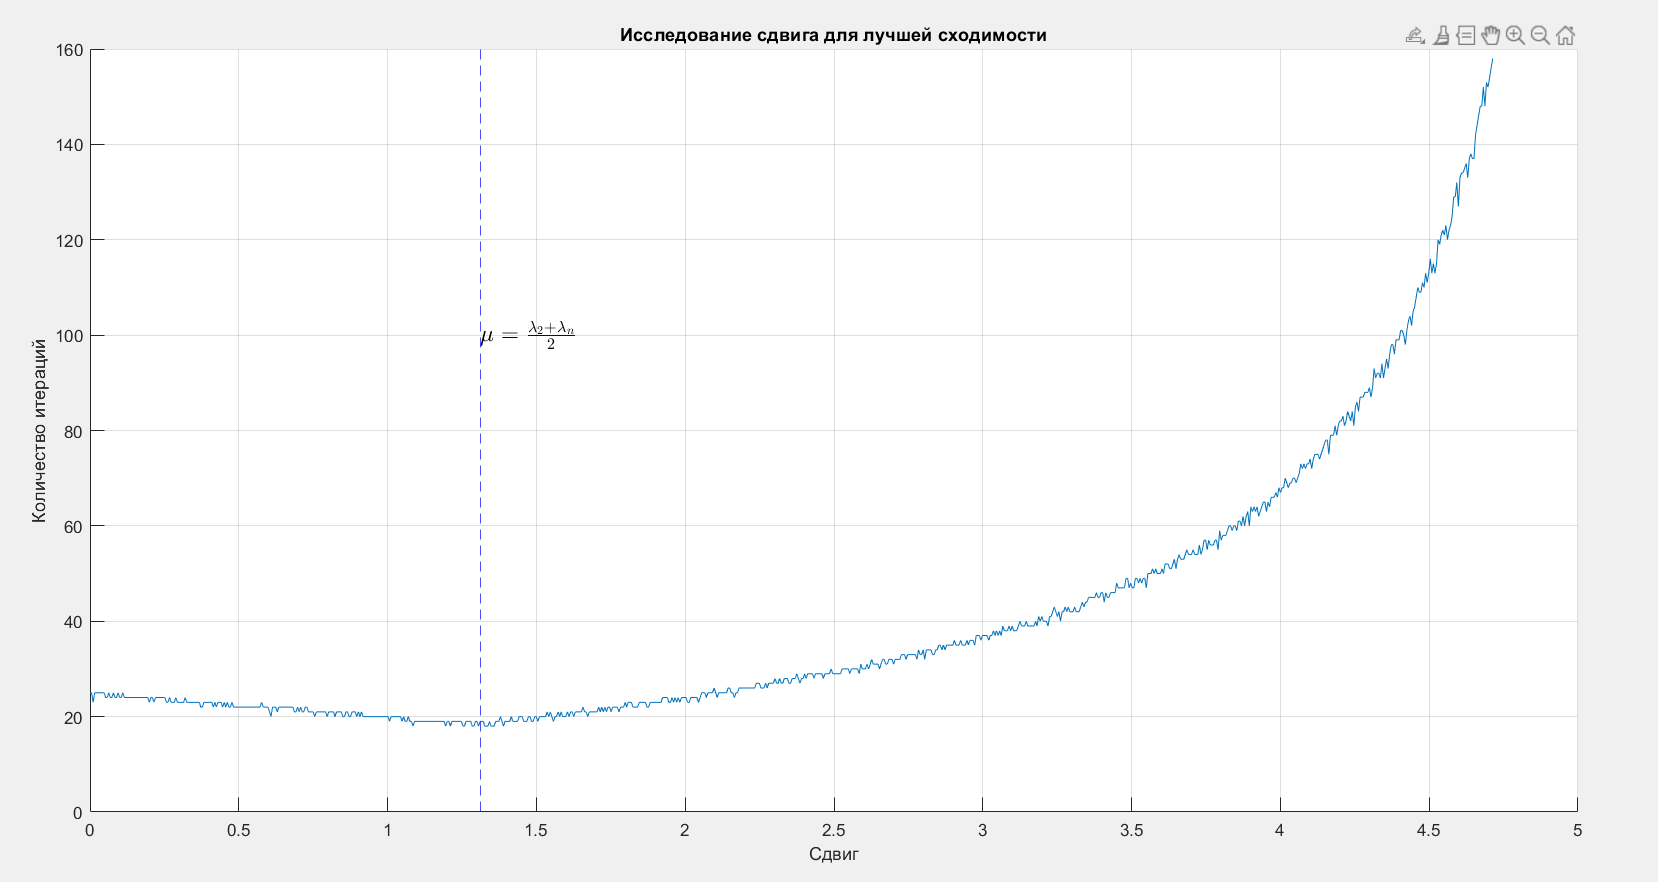
\includegraphics[scale = 0.4]{Сдвиг}\\
	Из графика видно, что при оптимальном сдвиге, наблюдается минимум количества итераций, что вполне логично и ожидаемо, ведь сдвиг оптимальный.\\
	\newpage
	$\triangleright$ \underline{Отделимость:}\\
	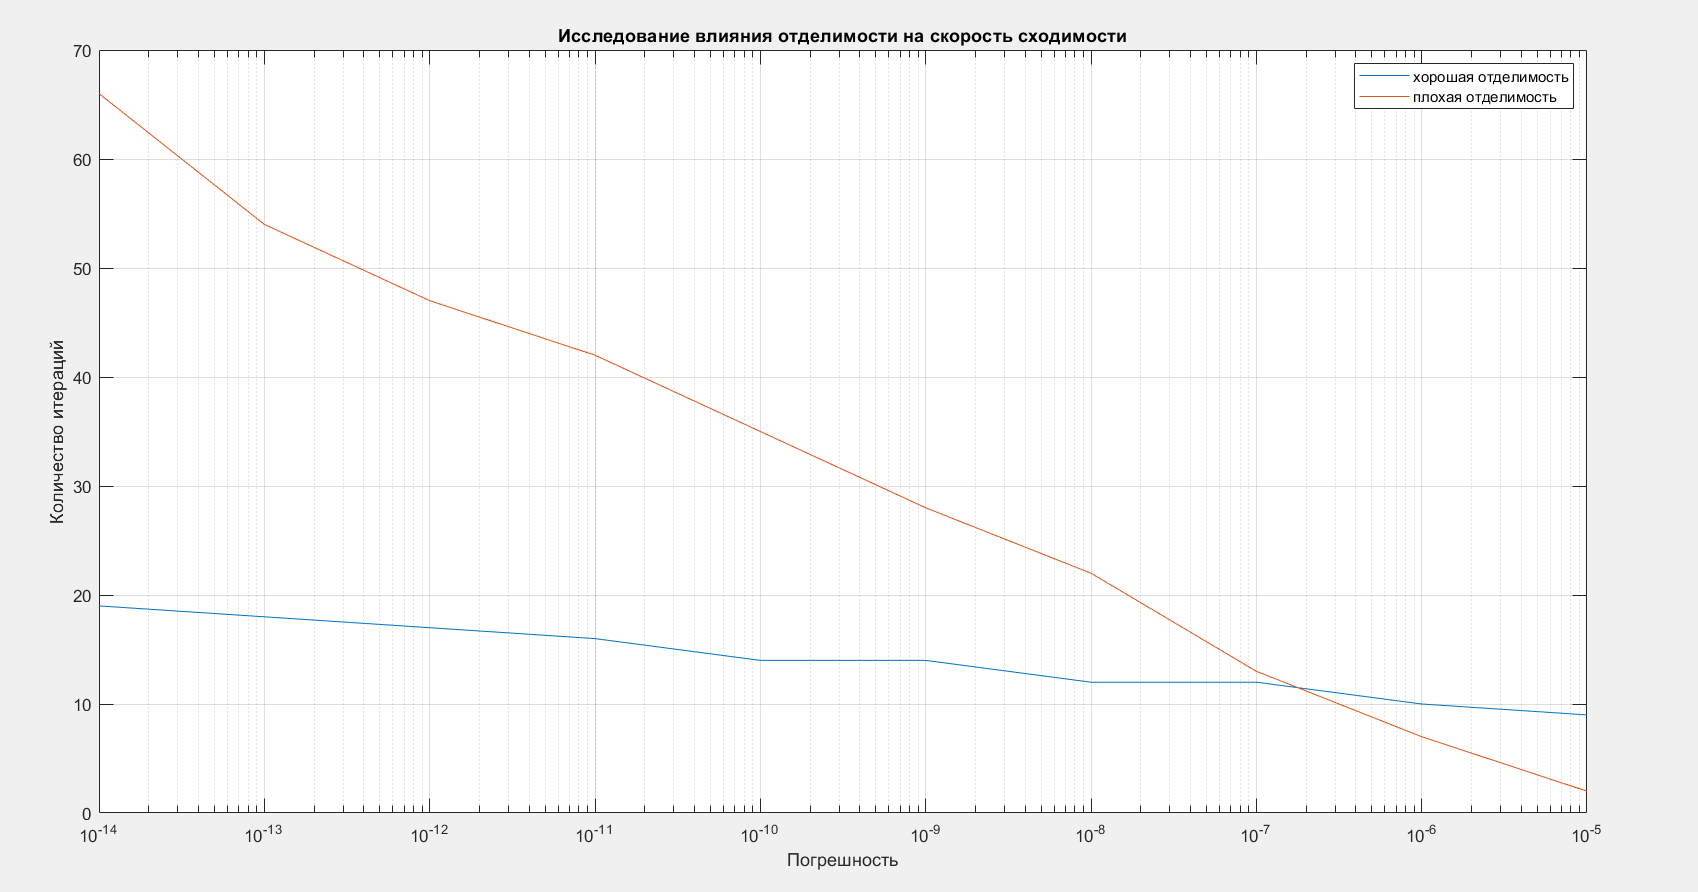
\includegraphics[scale = 0.4]{Отделимость}\\
	На графике мы видим, что при увеличении точности нужно совершить больше итераций для плохо отделимой матрицы, чтобы найти ее СЗ, для маленькой точности плохо отделимой матрице нужно всего 2 итерации, что объясняется тем, что беря произвольный исходный вектор, мы можем случайно близко попасть к искомому значению.\\
	$\triangleright$ \underline{Устойчивость АПСЗ:}\\
	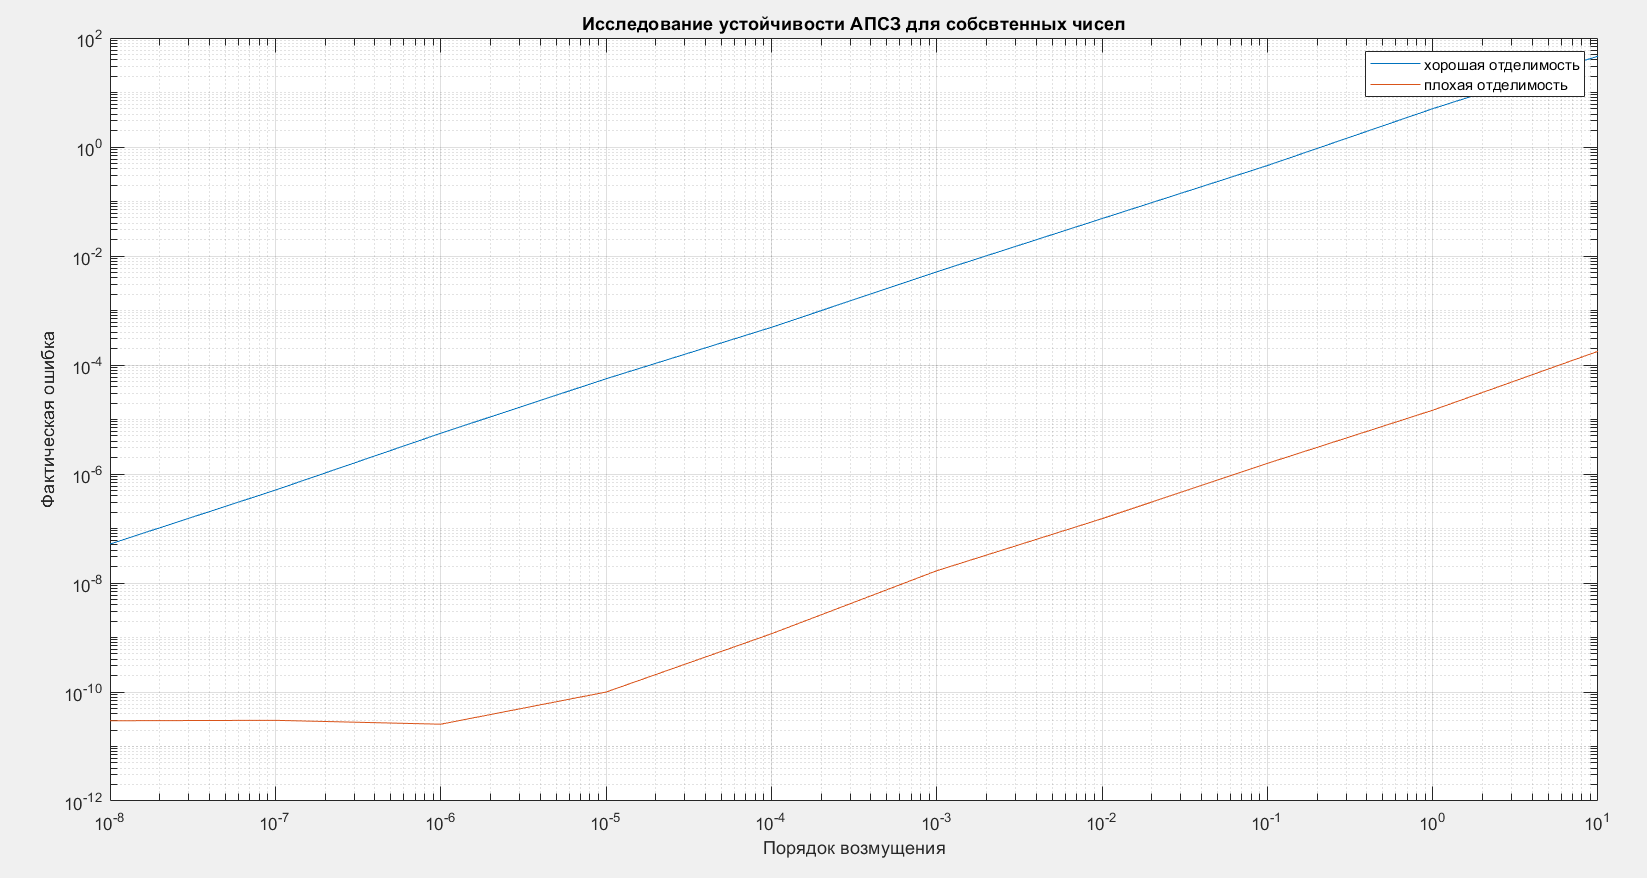
\includegraphics[scale = 0.255]{АПСЗ СЧ}
	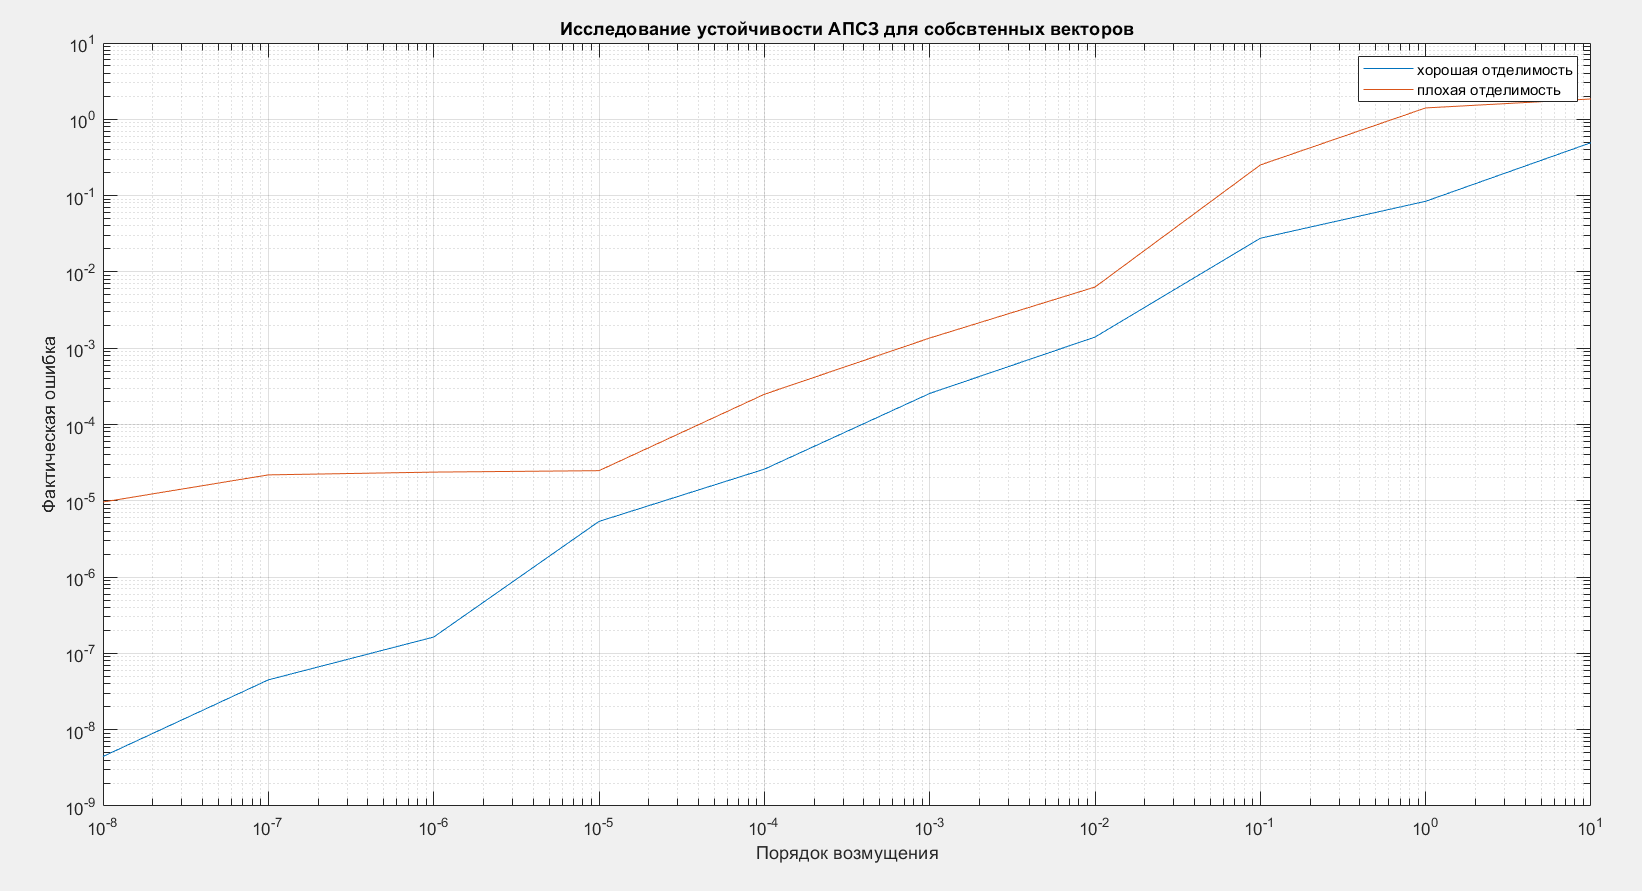
\includegraphics[scale = 0.25]{АПСЗ СВ}\\
	Из графиков становится очевидно, что при внесении достаточно большого возмущения, погрешность при нахождении СЗ так же возрастает, а промежуток между графиками возникает из-за сильного различия заданной отделимости.
	\begin{center} \textbf{Общие выводы:}\end{center}
	В данной лабораторной работе мы научились находить собственные значения матриц с помощью степенного метода. Мы увидели, что оптимальный сдвиг действительно оптимальный и что при преобладании максимального СЧ над другими, в частности, особенно над вторым максимальным СЧ, происходит ускорение сходимости метода.
\end{document}